\documentclass{beamer}

\usepackage[utf8]{inputenc}
\usepackage[english]{babel}
\usepackage[T1]{fontenc}
\usepackage{lmodern}
\usepackage{adjustbox}
\usepackage{graphicx}
\usepackage{caption}
\usepackage{subcaption}
\usepackage{color, colortbl}
\usepackage{commath}
\usepackage{amsmath,amssymb,amsthm}
\usepackage{tikz}
\usepackage{pgffor}
\usepackage[lined]{algorithm2e}
\usetheme{Singapore}
\newlength{\mylen}
\resetcounteronoverlays{compt}
\AtBeginSection[]
{
  \begin{frame}<beamer>
    \frametitle{Overview}
    \tableofcontents[currentsection]
  \end{frame}
}
\addtobeamertemplate{navigation symbols}{}{%
    \usebeamerfont{footline}%
    \usebeamercolor[fg]{footline}%
    \hspace{1em}%
    \insertframenumber/\inserttotalframenumber
}
\usepackage{upgreek}
\begin{document}

\title{Integrating lexical constraints to K-Means with Deep Learning}
\author{Maxence Grand \\                                                   
        Supervised by : Thibaut Thonet \and \'Eric Gaussier  \and Marc Tommasi \and Aur\'elien Bellet \and  Maziar Moradi Fard} 
\institute{Laboratoire d'Informatique de Grenoble, Team AMA}
\date{\today}

\maketitle

\begin{frame}{Overview}
\tableofcontents
\end{frame}
\section{Introduction}

\begin{frame}
\frametitle{$K$-Means}
Given a corpus C, where each document X is a 
N-dimensional real vector, k-means clustering aims to partition the n 
documents into K $S_k$ clusters represented by centroids 
R = {$r_1, r_2, ..., r_K$}. :
Formally, the objective is to minimize :
$$
\sum_{k =1 }^K \sum_{X \in S_k} ||X - r_k||_2^2
$$
\end{frame}

\foreach \n in {0,...,7}{
  \begin{frame}
    \frametitle{$K$-Means}
  \begin{figure}[!h]
    \centering
    \includegraphics[scale=0.45]{kmeans/\n test.png}
  \end{figure}
  \end{frame}
}

\begin{frame}
  \frametitle{Lexical Constraints}
  \pause
  \begin{itemize}
    \setlength\itemsep{2em}
  \item Set of keywords \pause
  \item Bias clustering
  \end{itemize}
\end{frame}

%Bas de page pour COP-KMeans et NNclust
\begin{frame}
\begin{itemize}
  \setlength\itemsep{1em}
\item Encode Function $h_{\theta}(X) = g(X; \theta)$
\item Decode Function $f(Y; \theta)$
\item $L_{rec}(X, \theta) = || X - f(h_{\theta}(X); \theta)||_2^2$
\end{itemize}
  \frametitle{Auto-Encoder}
  \begin{figure}[!h]
    \centering
    \fbox{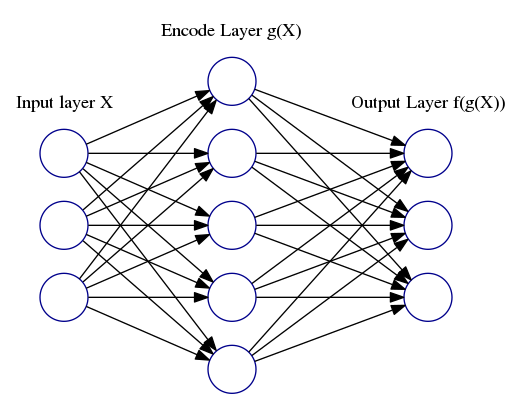
\includegraphics[scale=0.2]{autoencoder.png}}
    \label{fig:AE}
  \end{figure}
\end{frame}

\section{Proposed Method}

%Remplacer \Omega par L_{const}
\begin{frame}
\frametitle{The Idea}
Learn a latent space taking into account lexical constraints and
background knowledge.
\end{frame}

\begin{frame}
\frametitle{Lexical Constraints}
\begin{equation*}
  KW = \begin{pmatrix} kw_1 & kw_2 & ... & kw_{k-1} & kw_{k}
\end {pmatrix}
\end{equation*}
Introducing $X'$ such that a biasing version of X :
\begin{enumerate}
\item \textbf{Masked Document} :
\begin{equation*}
X_k' = mask_k(X) 
\end{equation*}
where $mask_k(X)$ is the document X masked by keywords from the $k^{th}$ class
\begin{equation*}
\forall i, mask_k(X)_i = \left\{
\begin{array}{ll}
  X_i & \mbox{if } i \in KW_k\\
  0 & \mbox{Otherwise.}
\end{array}
\right. 
\end{equation*}
\item \textbf{Similarity function} :
\begin{equation*}
   X'_k = \forall i, X_i \nu(i,k) 
\end{equation*}
\end{enumerate}
\end{frame}


\begin{frame}
  \frametitle{Deep $K$-Means }
  \resizebox{\hsize}{!}{
  \fbox{\includegraphics{approach_overview.pdf}}
  }
\end{frame}

\begin{frame}
  \frametitle{Deep $K$-Means }
\begin{equation*}
  L_{Clust}(C,\alpha;\theta,R) = \sum_{X \in C} ||h_\theta(X)-c(h_\theta(X); R)||_2^2
\end{equation*}
\begin{equation*}
  c(h_\theta(X); R) = argmin_{r \in R}||h_\theta(X) - r||_2^2
\end{equation*}
\end{frame}

\begin{frame}
  \frametitle{Deep $K$-Means }
\begin{equation*}
L_{Clust}(C, K, \alpha; \theta, R) = \sum_{X \in C} \sum_{k=1}^K ||h_{\theta}(X) - r_k||_2^2 G_{k, F}(h_{\theta}(X), \alpha; R)
\end{equation*}
\begin{equation*}
G_{k, F}(h_{\theta}(X), \alpha; R) = \frac{e^{-\alpha ||g(X, \theta) - r_k||_2^2}}
{\sum_{k' = 1}^K e^{-\alpha ||g(X, \theta) - r_k||_2^2}}
\end{equation*}
\end{frame}

\begin{frame}
\frametitle{Final Loss}
\end{frame}

\begin{frame}
\frametitle{Training Algorithm & Pretraining}
\end{frame}

\section{Experiment}

\begin{frame}
  \frametitle{Data}
  \begin{itemize}
    \setlength\itemsep{2em}
  \item 20 newsgroups
  \item RCV1 
  \end{itemize}
\end{frame}

\begin{frame}
\frametitle{Keywords Extraction}
\scalebox{.7}{
\begin{algorithm}[H]
  \SetKwInOut{Input}{input}
  \SetKwInOut{Output}{output}
  \Input{Corpus C, The number of keywords per classes $P$}
  \Output{KW}
  $KW \gets \{\}$\\
  \ForEach{Class $c_i \in C$}{
    $rank_i \gets [0 ... 0]$\\
    \ForEach{Document $X \in c_i$}{
      \ForEach{Word $w \in X$}{
        $rank_{i,w} \gets rank_{i,w} + TFIDF(w,X, C)$\\
      }
    }
  }
  \If{$Discriminating\_ Extraction$}{
    \ForEach{Class $c_i \in C$}{
      ${rank'}_i \gets rank_i - \sum\limits_{\forall c_j, c_j \neq c_i}rank_j$\\
    }
    $rank \gets rank'$
  }
  \ForEach{Class $c_i \in C$}{
    $KW \gets KW \cup \{\{w_1, w_2 ... w_P\} : \not\exists (v_1, v_2) | v_1 \not\in 
    \{w_1, w_2 ... w_P\}, v_2 \in \{w_1, w_2 ... w_P\}, rank_{i,v_1} \ge rank_{i,v_2}\}$\\
  }
  \Return{KW}
  \caption{\label{algo:gen_kw}Extract Keywords}
\end{algorithm}
}
\end{frame}

\begin{frame}
\frametitle{Metric}
\begin{itemize}
\item NMI
\item Accuracy
\item Adjusted Rand Index
\end{itemize}
\end{frame}

\begin{frame}
  \frametitle{Baseline Algorithm}
  \begin{enumerate}
  \item $K$-Means
  \item Deep $K$-Means algorithm
  \end{enumerate}
\end{frame}

\begin{frame}
  \frametitle{Baseline Algorithm}
  \begin{enumerate}
  \item $K$-Means
    \begin{enumerate}
    \item KM
    \item AE + KM SP
    \item AE + KM LP
    \end{enumerate}
  \item Deep $K$-Means algorithm
  \end{enumerate}
\end{frame}

\begin{frame}
  \frametitle{Results}
  \begin{table}
%The best result for each  metric/dataset is bold.}
\centering
\resizebox{\hsize}{!}{
\begin{tabular}{|l|l|l|l|}
    \hline
                      & ACC      &ARI       &NMI       \\ \hline
    $K$-Means         &$36.1\pm2.2$&$13.3\pm1.7$&$40.9\pm1.6$\\ \hline
    AE + KM, SP       &$53.1\pm2.3$&$35.0\pm1.4$&$49.3\pm1.0$\\ \hline
    Deep $K$-Means    &$54.9\pm1.7$&$37.6\pm1.1$&$51.6\pm0.6$\\ \hline
    AE + KM, LP mask  &\boldmath$67.1\pm4.5$&$37.6\pm5.1$&$39.8\pm3.9$\\ \hline
    AE + KM, LP sim   &$56.0\pm2.3$&$37.6\pm1.6$&$50.8\pm0.7$\\ \hline
       CDKM, LP mask  &$61.3\pm0.6$&\boldmath$41.2\pm0.8$&$52.7\pm0.5$\\ \hline
       CDKM, LP sim   &$60.6\pm1.3$&$40.5\pm1.3$&$53.0\pm0.8$\\ \hline
       CDKM, SP mask  &$60.2\pm1.8$&\boldmath$41.2\pm0.9$&\boldmath$53.5\pm0.5$\\ \hline
       CDKM, SP sim   &$60.5\pm1.2$&$40.7\pm0.8$&$52.9\pm0.5$\\ \hline
\end{tabular}
\begin{tabular}{|l|l|l|l|}
    \hline
                      & ACC      &ARI       &NMI       \\ \hline
    $K$-Means         &$33.1\pm2.7$&$ 8.7\pm1.3$&$26.3\pm1.6$\\ \hline
    AE + KM, SP       &$45.2\pm3.3$&$23.0\pm2.5$&$30.0\pm2.0$\\ \hline
    Deep $K$-Means    &$44.5\pm2.4$&$23.6\pm2.4$&$30.2\pm2.0$\\ \hline
    AE + KM, LP mask  &$45.9\pm2.2$&$24.0\pm1.8$&$31.8\pm1.5$\\ \hline
    AE + KM, LP sim   &$46.2\pm2.6$&$24.6\pm1.9$&$32.3\pm1.3$\\ \hline
       CDKM, LP mask  &$50.0\pm2.1$&$26.0\pm1.6$&$31.7\pm1.7$\\ \hline
       CDKM, LP sim   &$49.4\pm2.1$&$25.3\pm1.9$&$31.1\pm1.7$\\ \hline
       CDKM, SP mask  &$49.5\pm1.7$&$26.1\pm1.1$&$32.0\pm0.9$\\ \hline
       CDKM, SP sim   &$49.3\pm1.1$&$25.9\pm1.2$&$32.0\pm1.1$\\ \hline
\end{tabular}
}
\subcaption*{20 Newsgroups}
\resizebox{0.5\hsize}{!}{
\begin{tabular}{|l|l|l|l|}
    \hline
                      & ACC      &ARI       &NMI       \\ \hline
    $K$-Means         &$48.8\pm6.6$&$18.4\pm6.0$&$29.7\pm5.8$\\ \hline
    AE + KM, SP       &$51.3\pm3.5$&$17.5\pm5.8$&$24.5\pm5.1$\\ \hline
    Deep $K$-Means    &$54.4\pm4.9$&$23.9\pm3.5$&$29.6\pm3.6$\\ \hline
    AE + KM, LP mask  &$65.0\pm6.7$&$35.6\pm7.3$&$37.5\pm6.5$\\ \hline
    AE + KM, LP sim   &$62.7\pm6.1$&$35.1\pm5.7$&$38.4\pm4.1$\\ \hline
       CDKM, LP mask  &\boldmath$72.7\pm4.0$&\boldmath$43.8\pm5.4$&\boldmath$44.1\pm3.9$\\ \hline
       CDKM, LP sim   &$72.5\pm4.5$&$43.7\pm5.7$&$44.0\pm4.3$\\ \hline
       CDKM, SP mask  &$70.3\pm4.2$&$41.0\pm5.1$&$42.1\pm4.0$\\ \hline
       CDKM, SP sim   &$70.4\pm5.1$&$41.8\pm7.1$&$43.0\pm5.2$\\ \hline
\end{tabular}
}
\subcaption*{RCV1}
\end{table}
\end{frame}

\begin{frame}
  \frametitle{Results}
  
\begin{table}
%The best result for each  metric/dataset is bold.}
\centering
\resizebox{\hsize}{!}{
\begin{tabular}{|l|l|l|l|}
    \hline
                      & ACC      &ARI       &NMI       \\ \hline
    $K$-Means         &$36.1\pm2.2$&$13.3\pm1.7$&$40.9\pm1.6$\\ \hline
    Deep $K$-Means    &$54.9\pm1.7$&$37.6\pm1.1$&$51.6\pm0.6$\\ \hline
    AE + KM, LP mask  &\boldmath$67.1\pm4.5$&$37.6\pm5.1$&$39.8\pm3.9$\\ \hline
    AE + KM, LP sim   &$56.0\pm2.3$&$37.6\pm1.6$&$50.8\pm0.7$\\ \hline
       CDKM, LP mask  &$58.8\pm1.4$&$38.5\pm1.4$&$52.6\pm0.6$\\ \hline
       CDKM, LP sim   &\boldmath$60.1\pm2.1$&\boldmath$40.2\pm1.4$&\boldmath$52.8\pm1.0$\\ \hline
       CDKM, SP mask  &$58.9\pm2.0$&$38.9\pm1.6$&\boldmath$52.8\pm0.9$\\ \hline
       CDKM, SP sim   &$60.1\pm1.7$&$40.1\pm1.5$&$52.7\pm0.7$\\ \hline
\end{tabular}
\begin{tabular}{|l|l|l|l|}
    \hline
                      & ACC      &ARI       &NMI       \\ \hline
    $K$-Means         &$33.1\pm2.7$&$ 8.7\pm1.3$&$26.3\pm1.6$\\ \hline
    Deep $K$-Means    &$44.5\pm2.4$&$23.6\pm2.4$&$30.2\pm2.0$\\ \hline
    AE + KM, LP mask  &\boldmath$67.1\pm4.5$&$37.6\pm5.1$&$39.8\pm3.9$\\ \hline
    AE + KM, LP sim   &$56.0\pm2.3$&$37.6\pm1.6$&$50.8\pm0.7$\\ \hline
       CDKM, LP mask   &$48.8\pm2.3$&\boldmath$25.7\pm1.9$&\boldmath$31.6\pm1.9$\\ \hline
       CDKM, LP sim  &$47.8\pm2.6$&$24.3\pm1.8$&$30.8\pm1.7$\\ \hline
       CDKM, SP mask  &$48.8\pm2.3$&$25.7\pm1.9$&$31.6\pm1.9$\\ \hline
       CDKM, SP sim   &\boldmath$49.2\pm2.3$&$25.2\pm2.0$&$31.5\pm1.7$\\ \hline
\end{tabular}
}
\subcaption*{20 Newsgroups}
\resizebox{0.5\hsize}{!}{
\begin{tabular}{|l|l|l|l|}
    \hline
                      & ACC      &ARI       &NMI       \\ \hline
    $K$-Means         &$48.8\pm6.6$&$18.4\pm6.0$&$29.7\pm5.8$\\ \hline
    Deep $K$-Means    &$54.4\pm4.9$&$23.9\pm3.5$&$29.6\pm3.6$\\ \hline
    AE + KM, LP mask  &\boldmath$67.1\pm4.5$&$37.6\pm5.1$&$39.8\pm3.9$\\ \hline
    AE + KM, LP sim   &$56.0\pm2.3$&$37.6\pm1.6$&$50.8\pm0.7$\\ \hline
       CDKM, LP mask  &\boldmath$68.5\pm5.6$&\boldmath$39.6\pm6.4$&\boldmath$41.3\pm4.6$\\ \hline
       CDKM, LP sim   &$65.8\pm5.0$&$36.2\pm5.5$&$38.9\pm3.7$\\ \hline
       CDKM, SP mask  &$68.5\pm5.6$&$39.6\pm6.4$&$41.3\pm4.6$\\ \hline
       CDKM, SP sim   &$67.5\pm6.3$&$38.6\pm6.4$&$40.7\pm4.4$\\ \hline
\end{tabular}
}
\subcaption*{RCV1}
\end{table}
\end{frame}

\begin{frame}
  \frametitle{Results}
\begin{figure}
    \centering
    \fbox{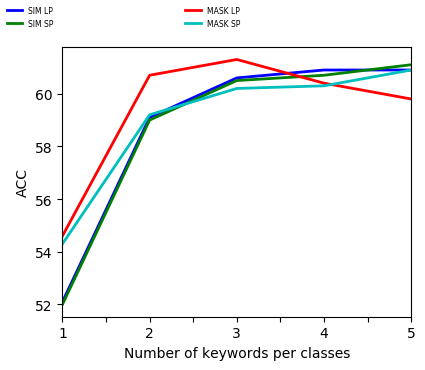
\includegraphics[scale=0.35]{res/dat_file/acc/20NEWS_ACC.png}}     
    \fbox{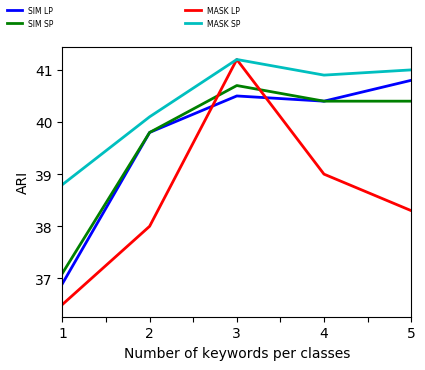
\includegraphics[scale=0.35]{res/dat_file/ari/20NEWS_ARI.png}}    
    \fbox{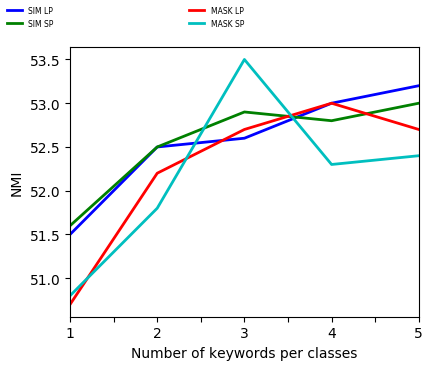
\includegraphics[scale=0.35]{res/dat_file/nmi/20NEWS_NMI.png}}    
\end{figure}
\end{frame}


\section{Conclusion \& Future Works}

\begin{frame}
  \frametitle{Conclusion \& Future Works}
\begin{itemize}
\item We have presented and tested in this study an approach to integrate lexical constraints to $K$-Means algorithm. \pause 
\item Future Works
\begin{itemize}
\item Test pairwise constraints
\item More baseline Algorithm
\begin{itemize}
\item COP$K$-Means
\item Deep COP$K$-Means
\end{itemize}
\item Robustness
\begin{itemize}
\item Change number of keywords
\item Change number of cluster
\end{itemize}
\end{itemize}
\end{itemize}
\end{frame}

\begin{frame}
Any Questions ?
\end{frame}

\begin{frame}
\frametitle{$G_{F,k}$ \& $\alpha$}
\begin{equation*}
G_{k, F}(h_{\theta}(X), \alpha; R) = \frac{e^{-\alpha ||h_\theta(X) - r_k||_2^2}}
{\sum_{k' = 1}^K e^{-\alpha ||g(X, \theta) - r_k||_2^2}}
\end{equation*}
\begin{equation*}
  \lim\limits_{\alpha \rightarrow \alpha_0}G_{k, F}(h_\theta(X), \alpha; R) = \left\{
\begin{array}{ll}
  1 & \mbox{if }r_k = c(h_\theta(X); R)\\
  0 & \mbox{Otherwise.}
\end{array}
\right.
\end{equation*}
where $\alpha$ play the role of an inverse temperature.
\end{frame}

\begin{frame}
\frametitle{Stochastic gradient descent (SGD)}
\begin{equation*}
  (\theta, R) \gets (\theta, R) - \epsilon \frac{1}{|\widetilde{C}|}
  \nabla_{(\theta, R)} L(C, \alpha; \theta, R)
\end{equation*}
where $\widetilde{C}$ is a random mini batch of C, and $\epsilon$ the
learning rate.
\end{frame}
\begin{frame}
\frametitle{Training dkm}
\scalebox{0.7}{
\begin{algorithm}[H]
  \SetKwInOut{Input}{input}
  \SetKwInOut{Output}{output}
  \Input{Corpus C , number of clusters K, balancing parameter $\lambda$,
    scheme for $\alpha$, number of epochs T ,
    number of minibatches MB , learning rate $\epsilon$}
  \Output{Auto-Encoder parameter $\theta$, cluster representative R}
  Initialise $\theta$ and $r_k$, $1 \leq k \leq K$ (randomly or through 
  pretraining)\\
  \ForEach{$\alpha = m_\alpha : M_\alpha$}{
    \ForEach{t = 1 : T}{
      \ForEach{n = 1 : MB}{
        Draw minibatch $\widetilde{C} \subseteq  C$\\
        Update ($\theta, R$) using SGD
      } 
    }  
  }
\end{algorithm}
}
\end{frame}

\begin{frame}
\frametitle{Metric - NMI}
The NMI Metric is defined as follows
$$NMI(S,C) = \frac{I(S,C)}{[H(S)+H(C)]/2}$$ 
with
$I(S,C) =\sum_k \sum_f\frac{|s_k \cap c_f|}{N}log\frac{N|s_k \cap c_f|}{|s_k| |c_f|}$
and
$H(S) = -\sum_k\frac{|s_k|}{N}log\frac{N|s_k|}{|s_k|}$
\end{frame}

\begin{frame}
\frametitle{Metric - Accuracy}
The Accuracy is the proportion of true results among the total
  number of cases examined. The Accuracy metric is defined as follows :
$$ACC(S,C) = \frac{1}{N}\sum_k {max}_j|s_k \cap c_j|$$
\end{frame}

\begin{frame}
\frametitle{Metric - Adjusted Rand Index}
Let a be the number of pairs of document in C
  that are in the same cluster in the predicted partition and in the
  same cluster in the real partition, and b be the number of pairs of
  document in C that are in different clusters in predicted partition
  and in different cluster in real partition.
  The Adjusted Rand index is defined as follows :
  $$ARI = \frac{a+b}{\binom{N}{2}}$$
\end{frame}

\begin{frame}
\frametitle{Architecture}
\begin{figure}[!h]
  \centering
  \fbox{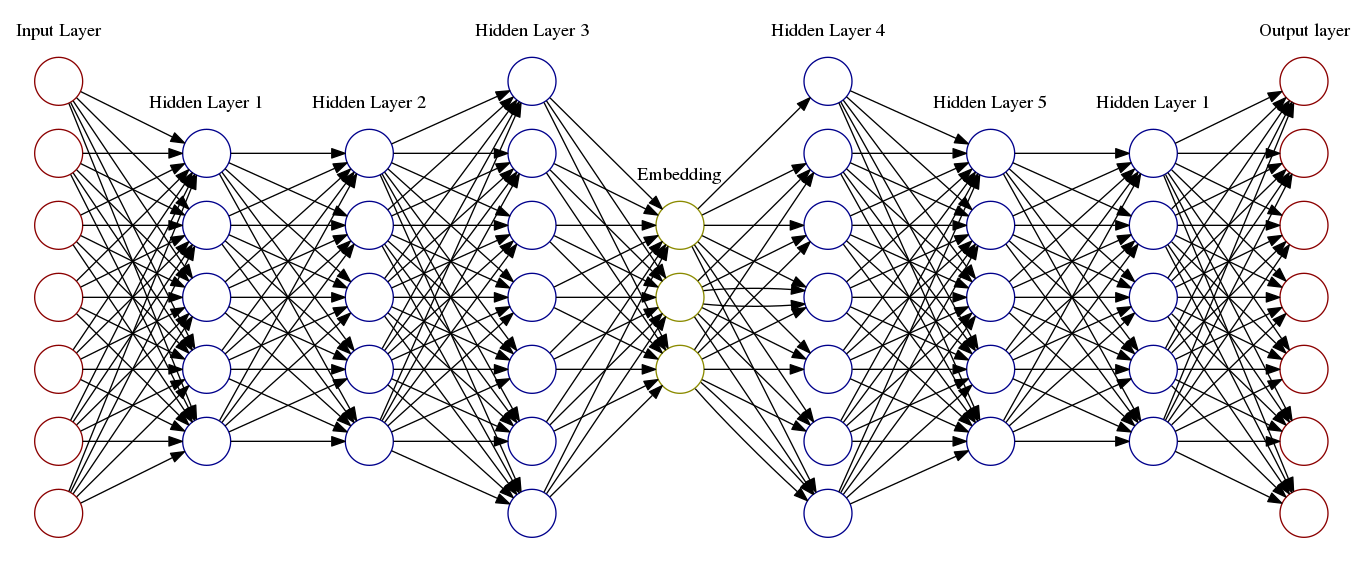
\includegraphics[scale=0.2]{archi.png}}
  \caption{\label{fig:archi}Architecture}
\end{figure}
\end{frame}

\begin{frame}
\frametitle{Hyperparameters}
Grid search on the set \{$10^i | i \in [-6, -1]$\}.
\begin{table}
\caption{\label{tab:line_search_met1}Best results of Grid Search for the optimization of
hyperparameters for each dataset.}
%The best result for each  metric/dataset is bold.}
\centering
\resizebox{.6\textwidth}{!}{
\begin{tabular}{|l|l|l|}
    \hline
                      &$\lambda_0$&$\lambda_1$       \\ \hline
    Deep $K$-Means    &$10^{-1}$  &\cellcolor{gray}         \\ \hline
    AE + KM, LP mask  &\cellcolor{gray}  &$10^{-2}$         \\ \hline
    AE + KM, LP sim   &\cellcolor{gray}  &$10^{-2}$         \\ \hline
       CDKM, LP mask  &$10^{-6}$  &$10^{-1}$         \\ \hline
       CDKM, LP sim   &$10^{-3}$  &$10^{-1}$         \\ \hline
       CDKM, SP mask  &$10^{-1}$  &$10^{-6}$         \\ \hline
       CDKM, SP sim   &$10^{-1}$  &$10^{-5}$         \\ \hline
\end{tabular}
\begin{tabular}{|l|l|l|}
    \hline
                      &$\lambda_0$&$\lambda_1$       \\ \hline
    Deep $K$-Means    &$10^{-1}$  &\cellcolor{gray}         \\ \hline
    AE + KM, LP mask  &\cellcolor{gray}  &$10^{-2}$         \\ \hline
    AE + KM, LP sim   &\cellcolor{gray}  &$10^{-2}$         \\ \hline
       CDKM, LP mask  &$10^{-1}$  &$10^{-3}$         \\ \hline
       CDKM, LP sim   &$10^{-1}$  &$10^{-3}$         \\ \hline
       CDKM, SP mask  &$10^{-1}$  &$10^{-4}$         \\ \hline
       CDKM, SP sim   &$10^{-1}$  &$10^{-5}$         \\ \hline
\end{tabular}
}
\subcaption*{20 Newsgroups}
\resizebox{.3\textwidth}{!}{
\begin{tabular}{|l|l|l|}
    \hline
                      &$\lambda_0$&$\lambda_1$       \\ \hline
    Deep $K$-Means    &$10^{-2}$  &\cellcolor{gray}         \\ \hline
    AE + KM, LP mask  &\cellcolor{gray}  &$10^{-4}$         \\ \hline
    AE + KM, LP sim   &\cellcolor{gray} &$10^{-2}$         \\ \hline
       CDKM, LP mask  &$10^{-1}$  &$10^{-3}$         \\ \hline
       CDKM, LP sim   &$10^{-1}$  &$10^{-3}$         \\ \hline
       CDKM, SP mask  &$10^{-1}$  &$10^{-3}$         \\ \hline
       CDKM, SP sim   &$10^{-1}$  &$10^{-2}$         \\ \hline
\end{tabular}
}
\subcaption*{RCV1}
\end{table}
\end{frame}

\end{document}
